% Chapter 1: Introduction and Data Sources
% Harvard-quality academic presentation
% Bachelor program, Bucharest University of Economic Studies

\documentclass[9pt, aspectratio=169, t]{beamer}

% Ensure content fits on slides
\setbeamersize{text margin left=8mm, text margin right=8mm}

%=============================================================================
% THEME AND STYLE CONFIGURATION
%=============================================================================
\usetheme{default}
% Using default theme for clean header/footer control

% Color Palette (matching Redispatch PDF)
\definecolor{MainBlue}{RGB}{26, 58, 110}
\definecolor{AccentBlue}{RGB}{26, 58, 110}
\definecolor{IDAred}{RGB}{205, 0, 0}
\definecolor{DarkGray}{RGB}{51, 51, 51}
\definecolor{MediumGray}{RGB}{128, 128, 128}
\definecolor{LightGray}{RGB}{248, 248, 248}
\definecolor{VeryLightGray}{RGB}{235, 235, 235}
\definecolor{KeynoteGray}{RGB}{218, 218, 218}
\definecolor{SectionGray}{RGB}{120, 120, 120}
\definecolor{FooterGray}{RGB}{100, 100, 100}
\definecolor{Crimson}{RGB}{220, 53, 69}
\definecolor{Forest}{RGB}{46, 125, 50}
\definecolor{Amber}{RGB}{181, 133, 63}
\definecolor{Orange}{RGB}{230, 126, 34}
\definecolor{Purple}{RGB}{142, 68, 173}

% Gradient background (exact Keynote 315° gradient: white to RGB 218,218,218)
\setbeamertemplate{background}{%
    \begin{tikzpicture}[remember picture, overlay]
        \shade[shading=axis, shading angle=315,
        top color=white, bottom color=KeynoteGray]
        (current page.south west) rectangle (current page.north east);
    \end{tikzpicture}%
}
% Fallback solid color for compatibility
\setbeamercolor{background canvas}{bg=}

\setbeamercolor{palette primary}{bg=MainBlue, fg=white}
\setbeamercolor{palette secondary}{bg=MainBlue!85, fg=white}
\setbeamercolor{palette tertiary}{bg=MainBlue!70, fg=white}
\setbeamercolor{structure}{fg=MainBlue}
\setbeamercolor{title}{fg=IDAred}
\setbeamercolor{frametitle}{fg=IDAred, bg=}
\setbeamercolor{block title}{bg=MainBlue, fg=white}
\setbeamercolor{block body}{bg=VeryLightGray, fg=DarkGray}
\setbeamercolor{block title alerted}{bg=Crimson, fg=white}
\setbeamercolor{block body alerted}{bg=Crimson!8, fg=DarkGray}
\setbeamercolor{block title example}{bg=Forest, fg=white}
\setbeamercolor{block body example}{bg=Forest!8, fg=DarkGray}
\setbeamercolor{item}{fg=MainBlue}

% Footer colors (override Madrid theme blue)
\setbeamercolor{author in head/foot}{fg=FooterGray, bg=}
\setbeamercolor{title in head/foot}{fg=FooterGray, bg=}
\setbeamercolor{date in head/foot}{fg=FooterGray, bg=}
\setbeamercolor{section in head/foot}{fg=FooterGray, bg=}
\setbeamercolor{subsection in head/foot}{fg=FooterGray, bg=}

% Bullet styles (apply everywhere including blocks)
\setbeamertemplate{itemize item}{\color{MainBlue}$\boxdot$}
\setbeamertemplate{itemize subitem}{\color{MainBlue}$\blacktriangleright$}
\setbeamertemplate{itemize subsubitem}{\color{MainBlue}\tiny$\bullet$}
\setbeamertemplate{itemize/enumerate body begin}{\normalsize}
\setbeamertemplate{itemize/enumerate subbody begin}{\normalsize}

% Item spacing - compact style
\setlength{\leftmargini}{10pt}       % Level 1: minimal indent
\setlength{\leftmarginii}{10pt}      % Level 2: minimal additional indent
% Compact list spacing (zero extra space before/after lists in blocks)
\makeatletter
\def\@listi{\leftmargin\leftmargini \topsep 0pt \parsep 0pt \itemsep 0pt}
\def\@listii{\leftmargin\leftmarginii \topsep 0pt \parsep 0pt \itemsep 0pt}
\makeatother

\setbeamertemplate{navigation symbols}{}

%=============================================================================
% CUSTOM HEADLINE
%=============================================================================
\setbeamertemplate{headline}{%
    \vskip10pt%
    \hbox to \paperwidth{%
        \hskip0.5cm%
        {\small\color{FooterGray}\renewcommand{\hyperlink}[2]{##2}\insertsectionhead}%
        \hfill%
        \textcolor{FooterGray}{\small\insertframenumber}%
        \hskip0.5cm%
    }%
    \vskip4pt%
    {\color{FooterGray}\hrule height 0.4pt}%
}

%=============================================================================
% CUSTOM FOOTER
%=============================================================================
\usepackage{fontawesome5}

\setbeamertemplate{footline}{%
    {\color{FooterGray}\hrule height 0.4pt}%
    \vskip4pt%
    \hbox to \paperwidth{%
        \hskip0.5cm%
        \textcolor{FooterGray}{\small Statistics of Financial Markets}%
        \hfill%
        \raisebox{-0.1em}{%
            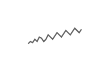
\begin{tikzpicture}[x=0.08em, y=0.08em, line width=0.4pt]
                \draw[FooterGray] (0,3) -- (1,4) -- (2,3.5) -- (3,5) -- (4,4) -- (5,6) -- (6,5.5) -- (7,4) -- (8,5) -- (9,7) -- (10,6) -- (11,5) -- (12,6.5) -- (13,8) -- (14,7) -- (15,6) -- (16,7.5) -- (17,9) -- (18,8) -- (19,7) -- (20,8.5) -- (21,10) -- (22,9) -- (23,8) -- (24,9.5);
            \end{tikzpicture}%
        }%
        \hskip0.5cm%
    }%
    \vskip6pt%
}

%=============================================================================
% PACKAGES
%=============================================================================
\usepackage[utf8]{inputenc}
\usepackage[T1]{fontenc}
\usepackage{amsmath, amssymb, amsthm}
\usepackage{mathtools}
\usepackage{bm}
\usepackage{tikz}
\usetikzlibrary{arrows.meta, positioning, shapes, calc, decorations.pathreplacing, shadings}
\usepackage{booktabs}
\usepackage{multirow}
\usepackage{array}
\usepackage{graphicx}
\usepackage{hyperref}
\usepackage{colortbl}
\usepackage{listings}
\lstset{language=Python, basicstyle=\ttfamily\scriptsize, keywordstyle=\color{MainBlue}\bfseries,
  commentstyle=\color{Forest}, stringstyle=\color{Crimson}, breaklines=true,
  frame=none, backgroundcolor=\color{VeryLightGray}, xleftmargin=2mm}
\hypersetup{colorlinks=true, linkcolor=MainBlue, urlcolor=MainBlue}
\graphicspath{{../../logos/}{../../charts/}{../../photos/}}
\hfuzz=2pt  % Suppress tiny overfull warnings (<2pt)
\vfuzz=2pt  % Suppress tiny vertical overfull warnings (<2pt)

%=============================================================================
% QUANTLET COMMAND
%=============================================================================
\newcommand{\quantlet}[2]{%
    \hfill\href{#2}{%
        \raisebox{-0.15em}{
\includegraphics[height=0.7em]{ql_logo.png}}%
        \textcolor{MainBlue}{\tiny\ #1}%
    }%
}

%=============================================================================
% CUSTOM TITLE PAGE
%=============================================================================
\defbeamertemplate*{title page}{hybrid}[1][]
{
    \vspace{0.2cm}
    % Logos row - top header (with clickable links)
    \begin{center}
        \href{https://www.ase.ro}{
\includegraphics[height=1.0cm]{ase_logo.png}}\hspace{0.3cm}%
        \href{https://theida.net}{
\includegraphics[height=1.0cm]{ida_logo.png}}\hspace{0.3cm}%
        \href{https://blockchain-research-center.com}{
\includegraphics[height=1.0cm]{brc_logo.png}}\hspace{0.3cm}%
        \href{https://www.ai4efin.ase.ro}{
\includegraphics[height=1.0cm]{ai4efin_logo.png}}\hspace{0.3cm}%
        \href{https://ipe.ro/new}{
\includegraphics[height=1.0cm]{acad_logo.png}}\hspace{0.3cm}%
        \href{https://www.digital-finance-msca.com}{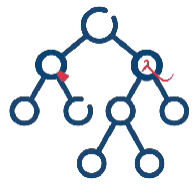
\includegraphics[height=1.0cm]{msca_logo.png}}%
    \end{center}

    \vspace{0.6cm}

    % Main title with Q logos on sides (with clickable links)
    \begin{center}
        \begin{minipage}{0.1\textwidth}
            \centering
            \href{https://quantlet.com}{
\includegraphics[height=1.1cm]{ql_logo.png}}
        \end{minipage}%
        \begin{minipage}{0.78\textwidth}
            \centering
            {\LARGE\bfseries\usebeamercolor[fg]{title}\inserttitle}

            \vspace{0.3cm}

            {\usebeamerfont{subtitle}\usebeamercolor[fg]{title}\insertsubtitle}
        \end{minipage}%
        \begin{minipage}{0.1\textwidth}
            \centering
            \href{https://quantinar.com}{
\includegraphics[height=1.1cm]{qr_logo.png}}
        \end{minipage}
    \end{center}

    \vspace{0.6cm}

    % Authors (left aligned)
    \hspace{0.5cm}{\usebeamerfont{author}\insertauthor}

    \vspace{0.3cm}

    % Institute/Affiliations (left aligned)
    \hspace{0.5cm}\begin{minipage}[t]{0.9\textwidth}
        \raggedright\small\insertinstitute
    \end{minipage}
}

%=============================================================================
% THEOREM ENVIRONMENTS
%=============================================================================
\theoremstyle{definition}
\setbeamertemplate{theorems}[numbered]
\newtheorem{defn}{Definition}
\newtheorem{thm}{Theorem}
\newtheorem{prop}{Proposition}
\newtheorem{rmk}{Remark}

%=============================================================================
% CENTRED MINIPAGE (no extra vertical space)
%=============================================================================
\newenvironment{cminipage}[1]{%
    \par\noindent\hfill\begin{minipage}{#1}\ignorespaces
}{%
    \end{minipage}\hfill\null\par
}

%=============================================================================
% CUSTOM COMMANDS
%=============================================================================
\newcommand{\E}{\mathbb{E}}
\newcommand{\Var}{\text{Var}}
\newcommand{\Cov}{\text{Cov}}
\newcommand{\Corr}{\text{Corr}}
\newcommand{\R}{\mathbb{R}}
\newcommand{\N}{\mathbb{N}}
\newcommand{\Z}{\mathbb{Z}}
\newcommand{\B}{\mathbf{B}}
\newcommand{\imark}{\textcolor{MainBlue}{\textbullet}}
\newcommand{\RMSE}{\text{RMSE}}
\newcommand{\MAE}{\text{MAE}}
\newcommand{\MAPE}{\text{MAPE}}

%=============================================================================
% TITLE INFORMATION
%=============================================================================
\title[Statistics of Financial Markets]{Statistics of Financial Markets}
\subtitle{Chapter 1: Introduction and Data Sources}
\author[D.T. Pele]{Daniel Traian PELE}
\institute{Bucharest University of Economic Studies\\
IDA Institute Digital Assets\\
Blockchain Research Center\\
AI4EFin Artificial Intelligence for Energy Finance\\
Romanian Academy, Institute for Economic Forecasting\\
MSCA Digital Finance}
\date{}

%=============================================================================
% BEGIN DOCUMENT
%=============================================================================
\begin{document}

%-----------------------------------------------------------------------------
% TITLE SLIDE
%-----------------------------------------------------------------------------
\begin{frame}[plain]
    \titlepage
\end{frame}

%#############################################################################
% SECTION: MOTIVATION
%#############################################################################
\section{Motivation}

%-----------------------------------------------------------------------------
% SLIDE 1: Why Data Matters
%-----------------------------------------------------------------------------
\begin{frame}{Why Data Matters}

\begin{itemize}
    \item Financial markets generate massive amounts of data every second.
    \item Understanding how to process, analyze, and interpret this data is key to making informed investment decisions.
    \item Data quality and selection directly impact model accuracy.
\end{itemize}

\vspace{0.4cm}

\begin{itemize}
    \item Understanding the Past
    \begin{itemize}
        \item Historical data helps us understand past market behavior.
        \item Identify trends.
        \item Analyze how markets have reacted to different events.
    \end{itemize}
    \item Predicting the Future
    \begin{itemize}
        \item Analyzing historical data can provide insights into potential future market movements.
        \item Inform investment decisions.
    \end{itemize}
\end{itemize}

\end{frame}

%-----------------------------------------------------------------------------
% SLIDE 2: Why Data Matters (continued)
%-----------------------------------------------------------------------------
\begin{frame}{Why Data Matters (continued)}

\begin{itemize}
    \item Understanding price data
    \begin{itemize}
        \item OHLC (Open, High, Low, Close) prices
        \item Adjusted close prices
    \end{itemize}
    \item Returns
    \begin{itemize}
        \item Simple returns
        \item Log-returns
        \item Cumulative returns
    \end{itemize}
    \item Volatility estimation
    \begin{itemize}
        \item Historical volatility
        \item Range-based estimators (Parkinson, Garman-Klass, Rogers-Satchell, Yang-Zhang)
    \end{itemize}
    \item Modern data challenges
    \begin{itemize}
        \item High-frequency data
        \item Alternative data sources
    \end{itemize}
\end{itemize}

\end{frame}

%-----------------------------------------------------------------------------
% SLIDE 3: Examples of Data Usage
%-----------------------------------------------------------------------------
\begin{frame}{Examples of Data Usage}

\begin{itemize}
    \item Stock Trading
    \begin{itemize}
        \item Price patterns, momentum strategies
        \item Traders use historical price and volume data to identify patterns and trends in the market.
    \end{itemize}
    \item Risk Management
    \begin{itemize}
        \item Value-at-Risk (VaR), stress testing
        \item Data is essential for quantifying and managing financial risks, such as market volatility, credit risk, and liquidity risk.
    \end{itemize}
    \item Portfolio Construction
    \begin{itemize}
        \item Correlation analysis, mean-variance optimization
        \item Quantitative analysts (quants) develop trading strategies and manage risk.
    \end{itemize}
    \item Algorithmic Trading
    \begin{itemize}
        \item Signals from statistical models
        \item Automated trading systems rely on real-time market data to execute trades at high speed.
    \end{itemize}
\end{itemize}

\end{frame}

%-----------------------------------------------------------------------------
% SLIDE 4: Data Challenges
%-----------------------------------------------------------------------------
\begin{frame}{Data Challenges}

\begin{itemize}
    \item Missing Data and Outliers
    \begin{itemize}
        \item Financial data can be noisy, incomplete, or inaccurate.
        \item Outliers may distort statistical estimates if not handled properly.
    \end{itemize}
    \item Survivorship Bias
    \begin{itemize}
        \item Databases often include only currently active securities, excluding delisted or bankrupt firms.
        \item This leads to overly optimistic performance estimates.
    \end{itemize}
    \item Look-Ahead Bias
    \begin{itemize}
        \item Using information that was not available at the time of the decision.
        \item Particularly dangerous in backtesting trading strategies.
    \end{itemize}
    \item Non-Stationarity
    \begin{itemize}
        \item Financial time series often exhibit time-varying statistical properties.
        \item Structural breaks, regime changes, and evolving market microstructure.
    \end{itemize}
    \item High-Frequency Noise
    \begin{itemize}
        \item Microstructure noise in tick-by-tick data.
        \item The sheer volume of financial data can be overwhelming.
    \end{itemize}
\end{itemize}

\end{frame}

%#############################################################################
% SECTION: PRICE DATA
%#############################################################################
\section{Price Data}

%-----------------------------------------------------------------------------
% SLIDE 5: Outline
%-----------------------------------------------------------------------------
\begin{frame}{Outline}

\begin{enumerate}
    \item Motivation \checkmark
    \item \textbf{Price Data}
    \item Returns
    \item Volatility Estimators
    \item Risk-Adjusted Returns
    \item Conclusions
    \item References
\end{enumerate}

\end{frame}

%-----------------------------------------------------------------------------
% SLIDE 6: OHLC Data
%-----------------------------------------------------------------------------
\begin{frame}{OHLC Data}

\begin{itemize}
    \item \textbf{O}pen Price $O_t$
    \begin{itemize}
        \item The first traded price at the beginning of the time period $t$.
        \item It reflects the initial market sentiment and can be influenced by news events occurring after the previous close.
    \end{itemize}
    \item \textbf{H}igh Price $H_t$
    \begin{itemize}
        \item The highest traded price during period $t$.
    \end{itemize}
    \item \textbf{L}ow Price $L_t$
    \begin{itemize}
        \item The lowest traded price during period $t$.
    \end{itemize}
    \item \textbf{C}lose Price $P_t$
    \begin{itemize}
        \item The last traded price at the end of period $t$.
        \item It is often considered the most significant price because it reflects the final consensus of value for that period.
    \end{itemize}
\end{itemize}

\vspace{0.3cm}
These four prices are the basic building blocks of financial data analysis.

\end{frame}

%-----------------------------------------------------------------------------
% SLIDE 7: Adjusted Close Price
%-----------------------------------------------------------------------------
\begin{frame}{Adjusted Close Price}

\begin{itemize}
    \item $P_t^{adj}$: accounts for corporate actions such as dividends, stock splits, and rights offerings that affect a stock's price but not its value.
    \item Ensures that historical price data reflects the true economic value of the stock over time, allowing for accurate performance analysis and comparison.
\end{itemize}

\vspace{0.2cm}
\textbf{Individual Adjustment Factors:}

\begin{itemize}
    \item \textbf{Stock Splits and Reverse Splits:} $F_i = \text{Split Ratio}_i$
    \item \textbf{Stock Dividends:} For a stock dividend of $d_i\%$: $F_i = 1 + d_i$
    \item \textbf{Cash Dividends:} $f_{\text{div}} = 1 - \dfrac{D}{P_{\text{close}}}$

    where $D_i$ is the cash dividend per share and $P_{i-1}$ is the close price before the dividend is paid.
    \item \textbf{Rights Offerings:} Shareholders can buy $n$ new shares at a subscription price $P_{\text{rights}}$ for every $m$ shares held:
    \[
    F_i = \frac{P_{i-1} + \left(\frac{n}{m} \times P_{\text{rights}}\right)}{P_{i-1}}
    \]
\end{itemize}

\vspace{0.2cm}
\textbf{Adjusted Price:} $\displaystyle P_t^{adj} = P_t \times \prod_{j} f_j$

\end{frame}

%#############################################################################
% SECTION: RETURNS
%#############################################################################
\section{Returns}

%-----------------------------------------------------------------------------
% SLIDE 8: Simple Returns
%-----------------------------------------------------------------------------
\begin{frame}{Simple Returns}

\begin{itemize}
    \item Return measures the gain or loss of an investment over a period, expressed as a percentage of the investment's initial cost.
\end{itemize}

\vspace{0.3cm}

\begin{defn}[Simple Return]
The \textbf{simple return} (or arithmetic return) of an asset over one period is defined as:
\[
R_t = \frac{P_t - P_{t-1}}{P_{t-1}} = \frac{P_t}{P_{t-1}} - 1
\]
where $P_t$ is the price at time $t$.
\end{defn}

\vspace{0.3cm}

\begin{itemize}
    \item Simple returns are intuitive and directly represent the percentage change in price.
    \item However, they are \textbf{not time-additive}: the multi-period simple return is a product, not a sum.
    \item Portfolio return: $R_p = \sum_{i=1}^{n} w_i R_i$ (simple returns aggregate across assets).
\end{itemize}

\end{frame}

%-----------------------------------------------------------------------------
% SLIDE 9: Log-Returns
%-----------------------------------------------------------------------------
\begin{frame}{Log-Returns}

\begin{defn}[Log-Return]
The \textbf{log-return} (or continuously compounded return) is defined as:
\[
r_t = \ln\left(\frac{P_t}{P_{t-1}}\right) = \ln P_t - \ln P_{t-1} = \ln(1 + R_t)
\]
\end{defn}

\vspace{0.3cm}

\textbf{Time-additivity property:}
\[
r_t(k) = r_t + r_{t-1} + \cdots + r_{t-k+1}
\]

\vspace{0.3cm}

\begin{itemize}
    \item For small changes in price: $r_t \approx R_t$.
    \item Under certain conditions, log-returns are more likely to follow a normal distribution.
    \item Log-returns simplify the mathematical handling of compounded returns.
    \item Enable more convenient statistical analysis, especially in the context of portfolio management and risk analysis.
\end{itemize}

\end{frame}

%-----------------------------------------------------------------------------
% SLIDE 10: Cumulative Returns
%-----------------------------------------------------------------------------
\begin{frame}{Cumulative Returns}

\begin{itemize}
    \item Cumulative returns represent the total change in the value of an investment over a period.
    \item Can be calculated using either simple returns or log-returns.
\end{itemize}

\vspace{0.3cm}

\textbf{Cumulative Simple Return (CSR):}
\[
\text{CSR}_T = \prod_{t=1}^{T}(1+R_t) - 1
\]

\vspace{0.3cm}

\textbf{Cumulative Log-Return (CLR):}
\[
\text{CLR}_T = \sum_{t=1}^{T} r_t
\]

\vspace{0.3cm}

\begin{itemize}
    \item The relationship between CSR and CLR: $\text{CSR}_T = e^{\text{CLR}_T} - 1$.
    \item CLR is simply the sum of individual log-returns (time-additivity).
    \item CSR requires multiplicative compounding of $(1+R_t)$ terms.
\end{itemize}

\quantlet{SFM\_ch1\_returns}{https://github.com/QuantLet/SFM/tree/main/SFM_ch1/SFM_ch1_returns}
\end{frame}

%#############################################################################
% SECTION: VOLATILITY ESTIMATORS
%#############################################################################
\section{Volatility Estimators}

%-----------------------------------------------------------------------------
% SLIDE 11: Volatility Overview
%-----------------------------------------------------------------------------
\begin{frame}{Volatility Overview}

\begin{itemize}
    \item Volatility is a statistical measure of the dispersion of returns for a given security or market index.
    \item It represents the degree of variation of an asset's price over time.
    \item Several estimators have been developed to capture the complexities of financial market volatility.
\end{itemize}

\vspace{0.3cm}

\begin{columns}[T]
\begin{column}{0.48\textwidth}
\textbf{Close-to-Close Estimators:}
\begin{itemize}
    \item Historical Volatility
\end{itemize}

\vspace{0.2cm}

\textbf{Range-Based Estimators:}
\begin{itemize}
    \item Parkinson's Estimator
    \item Garman-Klass Estimator
    \item Rogers-Satchell Estimator
    \item Yang-Zhang Estimator
\end{itemize}
\end{column}
\begin{column}{0.48\textwidth}
\textbf{Model-Based Estimators:}
\begin{itemize}
    \item Realized Volatility
    \item GARCH Models
    \item HEAVY Models
    \item Stochastic Volatility Models with Jumps
    \item Implied Volatility
\end{itemize}
\end{column}
\end{columns}

\end{frame}

%-----------------------------------------------------------------------------
% SLIDE 12: Historical Volatility
%-----------------------------------------------------------------------------
\begin{frame}{Historical Volatility}

\begin{itemize}
    \item Measures the dispersion or variability of returns over a specified period in the past.
    \item Uses closing prices only.
\end{itemize}

\vspace{0.3cm}

\begin{defn}[Historical Volatility]
Historical volatility is calculated as the standard deviation of past returns:
\[
\hat{\sigma} = \sqrt{\frac{1}{n-1}\sum_{i=1}^{n}(r_i - \bar{r})^2}
\]
where $r_i$ are the log-returns and $\bar{r}$ is the sample mean of returns.
\end{defn}

\vspace{0.3cm}

\begin{itemize}
    \item Limitations of Historical Volatility
    \begin{itemize}
        \item Past performance may not predict future volatility.
        \item Does not account for shocks or market regime changes.
        \item Ignores intra-day price information (High, Low, Open).
    \end{itemize}
\end{itemize}

\end{frame}

%-----------------------------------------------------------------------------
% SLIDE 13: Square Root of Time Rule
%-----------------------------------------------------------------------------
\begin{frame}{Square Root of Time Rule}

\begin{itemize}
    \item Fundamental concept in financial risk management and quantitative finance.
    \item Provides a method for scaling volatility (or risk) over different time horizons, assuming that returns are IID and follow a normal distribution.
\end{itemize}

\vspace{0.2cm}

Suppose we have an asset with returns $r_t \sim \mathcal{N}(\mu, \sigma^2)$ i.i.d. The total return over $n$ periods is:
\[
R_n = r_1 + r_2 + \ldots + r_n
\]

Since the returns are IID: $\E[R_n] = n\mu$ and $\Var(R_n) = n\sigma^2$.

\vspace{0.2cm}

The standard deviation (volatility) over $n$ periods is therefore:
\[
\sigma_n = \sqrt{\Var(R_n)} = \sqrt{n}\,\sigma
\]

\vspace{0.2cm}

\textbf{Annualized volatility} (Bachelier):
\[
\boxed{\sigma_{\text{annual}} = \sigma_{\text{daily}} \times \sqrt{252}}
\]
where 252 is the typical number of trading days in a year.

\end{frame}

%-----------------------------------------------------------------------------
% SLIDE 14: Parkinson's Estimator
%-----------------------------------------------------------------------------
\begin{frame}{Parkinson's Estimator}

\begin{itemize}
    \item Traditional estimators often rely solely on closing prices, potentially overlooking valuable information contained within the trading period.
    \item Parkinson (1980) introduced an estimator that utilizes the high and low prices within a period, offering a more efficient volatility estimate under specific assumptions.
    \item Assumptions: continuous trading, zero drift in the price process.
\end{itemize}

\vspace{0.3cm}

\begin{defn}[Parkinson's Estimator]
\[
\hat{\sigma}_P^2 = \frac{1}{4n\ln 2}\sum_{i=1}^{n}(\ln H_i - \ln L_i)^2
\]
where $H_i$ is the highest price on day $i$, $L_i$ is the lowest price on day $i$, and $n$ is the number of periods.
\end{defn}

\vspace{0.3cm}

\begin{itemize}
    \item Uses high-low range, more efficient than close-to-close estimators.
    \item Captures intra-period price variability more effectively.
\end{itemize}

\end{frame}

%-----------------------------------------------------------------------------
% SLIDE 15: Garman-Klass Estimator
%-----------------------------------------------------------------------------
\begin{frame}{Garman-Klass Estimator}

\begin{itemize}
    \item Garman and Klass (1980) extended the Parkinson estimator by incorporating open and close prices in addition to high and low prices.
\end{itemize}

\vspace{0.2cm}

\begin{defn}[Garman-Klass Estimator]
\[
\hat{\sigma}_{GK}^2 = \frac{1}{n}\sum_{i=1}^{n}\left[\frac{1}{2}(h_i - l_i)^2 - (2\ln 2 - 1)c_i^2\right]
\]
where:
\begin{itemize}
    \item $h_i = \ln H_i - \ln O_i$ (log high-to-open)
    \item $l_i = \ln L_i - \ln O_i$ (log low-to-open)
    \item $c_i = \ln C_i - \ln O_i$ (log close-to-open)
\end{itemize}
\end{defn}

\vspace{0.2cm}

\begin{columns}[T]
\begin{column}{0.48\textwidth}
\textbf{Advantages:}
\begin{itemize}
    \item Most efficient estimator under GBM assumptions
    \item Uses all four OHLC prices
    \item Approximately 8x more efficient than close-to-close
\end{itemize}
\end{column}
\begin{column}{0.48\textwidth}
\textbf{Limitations:}
\begin{itemize}
    \item Assumes zero drift
    \item Assumes continuous trading (no gaps)
    \item Sensitive to overnight price jumps
\end{itemize}
\end{column}
\end{columns}

\end{frame}

%-----------------------------------------------------------------------------
% SLIDE 16: Rogers-Satchell Estimator
%-----------------------------------------------------------------------------
\begin{frame}{Rogers-Satchell Estimator}

\begin{itemize}
    \item Rogers and Satchell (1991) developed an estimator that allows for non-zero drift in the price process, addressing a key limitation of Parkinson and Garman-Klass estimators.
\end{itemize}

\vspace{0.3cm}

\begin{defn}[Rogers-Satchell Estimator]
\[
\hat{\sigma}_{RS}^2 = \frac{1}{n}\sum_{i=1}^{n}\bigl[h_i(h_i - c_i) + l_i(l_i - c_i)\bigr]
\]
where:
\begin{itemize}
    \item $h_i = \ln H_i - \ln O_i$
    \item $l_i = \ln L_i - \ln O_i$
    \item $c_i = \ln C_i - \ln O_i$
\end{itemize}
\end{defn}

\vspace{0.3cm}

\begin{itemize}
    \item Allows for non-zero drift (trending markets).
    \item Uses all four OHLC prices.
    \item More robust than Parkinson and Garman-Klass in trending markets.
    \item Still assumes continuous trading (no overnight jumps).
\end{itemize}

\end{frame}

%-----------------------------------------------------------------------------
% SLIDE 17: Yang-Zhang Estimator
%-----------------------------------------------------------------------------
\begin{frame}{Yang-Zhang Estimator}

\begin{itemize}
    \item Yang and Zhang (2000) proposed the most comprehensive range-based volatility estimator, combining overnight volatility, open-to-close volatility, and the Rogers-Satchell estimator.
\end{itemize}

\vspace{0.2cm}

\begin{defn}[Yang-Zhang Estimator]
\[
\hat{\sigma}_{YZ}^2 = \hat{\sigma}_O^2 + k\,\hat{\sigma}_C^2 + (1-k)\,\hat{\sigma}_{RS}^2
\]
where:
\begin{itemize}
    \item $\hat{\sigma}_O^2$: overnight (close-to-open) variance
    \item $\hat{\sigma}_C^2$: open-to-close variance
    \item $\hat{\sigma}_{RS}^2$: Rogers-Satchell variance
    \item $k = \dfrac{0.34}{1.34 + \dfrac{n+1}{n-1}}$
\end{itemize}
\end{defn}

\vspace{0.2cm}

\begin{itemize}
    \item Most comprehensive range-based estimator.
    \item Handles both drift and opening jumps.
    \item Minimum variance estimator among range-based methods.
    \item Particularly useful for markets with significant overnight gaps.
\end{itemize}

\quantlet{SFM\_ch1\_volatility\_estimators}{https://github.com/QuantLet/SFM/tree/main/SFM_ch1/SFM_ch1_volatility_estimators}
\end{frame}

%#############################################################################
% SECTION: RISK-ADJUSTED RETURNS
%#############################################################################
\section{Risk-Adjusted Returns}

%-----------------------------------------------------------------------------
% SLIDE 18: Sharpe Ratio
%-----------------------------------------------------------------------------
\begin{frame}{Sharpe Ratio}

\begin{itemize}
    \item The Sharpe Ratio is the most widely used measure of risk-adjusted return.
    \item Developed by William F. Sharpe (1966), Nobel Laureate in Economics.
\end{itemize}

\vspace{0.3cm}

\begin{defn}[Sharpe Ratio]
\[
SR = \frac{E[R_p] - R_f}{\sigma_p}
\]
where:
\begin{itemize}
    \item $E[R_p]$: expected return of the portfolio
    \item $R_f$: risk-free rate
    \item $\sigma_p$: standard deviation of the portfolio's excess return
\end{itemize}
\end{defn}

\vspace{0.3cm}

\begin{itemize}
    \item Measures the excess return per unit of risk.
    \item Higher Sharpe Ratio indicates better risk-adjusted performance.
    \item Assumes returns are normally distributed.
    \item Widely used for comparing funds, strategies, and portfolios.
\end{itemize}

\end{frame}

%-----------------------------------------------------------------------------
% SLIDE 19: Interpreting the Sharpe Ratio
%-----------------------------------------------------------------------------
\begin{frame}{Interpreting the Sharpe Ratio}

\begin{center}
\renewcommand{\arraystretch}{1.6}
\begin{tabular}{>{\centering\arraybackslash}m{3.5cm} >{\centering\arraybackslash}m{4cm} >{\centering\arraybackslash}m{5cm}}
\toprule
\textbf{Sharpe Ratio} & \textbf{Rating} & \textbf{Interpretation} \\
\midrule
\cellcolor{Crimson!20} $SR < 0$ & \cellcolor{Crimson!20}\textcolor{Crimson}{\textbf{Bad}} & \cellcolor{Crimson!20} Returns below risk-free rate \\
\cellcolor{Orange!20} $0 \leq SR < 0.5$ & \cellcolor{Orange!20}\textcolor{Orange}{\textbf{Below Average}} & \cellcolor{Orange!20} Insufficient compensation for risk \\
\cellcolor{Amber!20} $0.5 \leq SR < 1.0$ & \cellcolor{Amber!20}\textcolor{Amber}{\textbf{Good}} & \cellcolor{Amber!20} Adequate risk-adjusted return \\
\cellcolor{Forest!15} $1.0 \leq SR < 2.0$ & \cellcolor{Forest!15}\textcolor{Forest}{\textbf{Very Good}} & \cellcolor{Forest!15} Strong risk-adjusted performance \\
\cellcolor{Forest!30} $SR \geq 2.0$ & \cellcolor{Forest!30}\textcolor{Forest!80!black}{\textbf{Excellent}} & \cellcolor{Forest!30} Exceptional (rare in practice) \\
\bottomrule
\end{tabular}
\end{center}

\vspace{0.4cm}

\begin{itemize}
    \item Most hedge funds and mutual funds have Sharpe Ratios between 0.5 and 1.5.
    \item A Sharpe Ratio above 2.0 is extremely rare over long time horizons.
\end{itemize}

\end{frame}

%-----------------------------------------------------------------------------
% SLIDE 20: Mathematical Framework
%-----------------------------------------------------------------------------
\begin{frame}{Mathematical Framework}

\textbf{Portfolio Expected Return:}

\vspace{0.2cm}

For a portfolio with $n$ assets and weights $w_1, w_2, \ldots, w_n$:
\[
E[R_p] = \sum_{i=1}^{n} w_i\, E[R_i]
\]
where:
\begin{itemize}
    \item $w_i$: weight of asset $i$ in the portfolio (with $\sum_{i=1}^n w_i = 1$)
    \item $E[R_i]$: expected return of asset $i$
\end{itemize}

\vspace{0.3cm}

\begin{itemize}
    \item The portfolio return is a linear combination of individual asset returns.
    \item Weights can be positive (long positions) or negative (short positions).
    \item In practice, expected returns are estimated from historical data or forward-looking models.
\end{itemize}

\end{frame}

%-----------------------------------------------------------------------------
% SLIDE 21: Portfolio Volatility
%-----------------------------------------------------------------------------
\begin{frame}{Portfolio Volatility}

\textbf{Portfolio Variance (scalar form):}
\[
\sigma_p^2 = \sum_{i=1}^{n}\sum_{j=1}^{n} w_i\, w_j\, \sigma_i\, \sigma_j\, \rho_{ij}
\]
where:
\begin{itemize}
    \item $\sigma_i$: standard deviation of asset $i$
    \item $\rho_{ij}$: correlation between assets $i$ and $j$
\end{itemize}

\vspace{0.3cm}

\textbf{Portfolio Volatility:}
\[
\sigma_p = \sqrt{\sum_{i=1}^{n}\sum_{j=1}^{n} w_i\, w_j\, \sigma_i\, \sigma_j\, \rho_{ij}}
\]

\vspace{0.3cm}

\textbf{Matrix notation:}
\[
\boxed{\sigma_p = \sqrt{\mathbf{w}^T \Sigma\, \mathbf{w}}}
\]
where $\mathbf{w}$ is the vector of portfolio weights and $\Sigma$ is the covariance matrix.

\vspace{0.2cm}

\begin{itemize}
    \item Diversification reduces portfolio volatility when $\rho_{ij} < 1$.
\end{itemize}

\end{frame}

%-----------------------------------------------------------------------------
% SLIDE 22: Portfolio Optimization
%-----------------------------------------------------------------------------
\begin{frame}{Portfolio Optimization}

\textbf{Efficient Frontier (Markowitz, 1952):}

\vspace{0.3cm}

\begin{itemize}
    \item \textbf{Maximize return for given risk:}
    \[
    \max_{\mathbf{w}} \quad \mathbf{w}^T \boldsymbol{\mu} \quad \text{s.t.} \quad \mathbf{w}^T \Sigma\, \mathbf{w} = \sigma_0^2, \quad \mathbf{w}^T \mathbf{1} = 1
    \]
    \item \textbf{Minimize risk for given return:}
    \[
    \min_{\mathbf{w}} \quad \mathbf{w}^T \Sigma\, \mathbf{w} \quad \text{s.t.} \quad \mathbf{w}^T \boldsymbol{\mu} = \mu_0, \quad \mathbf{w}^T \mathbf{1} = 1
    \]
\end{itemize}

\vspace{0.3cm}

\begin{itemize}
    \item The efficient frontier represents the set of portfolios offering the highest expected return for each level of risk.
    \item Portfolios below the efficient frontier are suboptimal (dominated).
    \item The minimum variance portfolio lies at the leftmost point of the frontier.
    \item The tangency portfolio maximizes the Sharpe Ratio.
\end{itemize}

\end{frame}

%-----------------------------------------------------------------------------
% SLIDE 23: Efficient Frontier -- Example
%-----------------------------------------------------------------------------
\begin{frame}{Efficient Frontier -- Example}

\textbf{Asset Universe:} SPY, QQQ, GLD, TLT, VNQ

\vspace{0.2cm}

\begin{center}
\renewcommand{\arraystretch}{1.3}
\scriptsize
\begin{tabular}{lccc}
\toprule
\textbf{Asset} & \textbf{Ann. Return (\%)} & \textbf{Ann. Volatility (\%)} & \textbf{Sharpe Ratio} \\
\midrule
SPY & 14.33 & 19.35 & 0.6370 \\
QQQ & 19.57 & 24.04 & 0.7309 \\
GLD & 11.62 & 14.31 & 0.6725 \\
TLT & $-0.37$ & 16.16 & $-0.1469$ \\
VNQ & 8.23 & 22.75 & 0.2738 \\
\bottomrule
\end{tabular}
\end{center}

\vspace{0.2cm}

\begin{itemize}
    \item Data period: 2018-01-01 to 2025-03-04 (1801 trading days).
    \item 10,000 random portfolios generated to illustrate the efficient frontier.
    \item QQQ has the highest return but also the highest volatility.
    \item GLD offers the best diversification benefit (lowest volatility, decent Sharpe).
    \item TLT has a negative Sharpe Ratio, reflecting the bond bear market.
    \item The optimal portfolio (maximum Sharpe) typically overweights QQQ and GLD.
\end{itemize}

\quantlet{SFM\_ch1\_sharpe\_ratio}{https://github.com/QuantLet/SFM/tree/main/SFM_ch1/SFM_ch1_sharpe_ratio}
\end{frame}

%#############################################################################
% SECTION: CONCLUSIONS
%#############################################################################
\section{Conclusions}

%-----------------------------------------------------------------------------
% SLIDE 24: Summary
%-----------------------------------------------------------------------------
\begin{frame}{Summary}

\begin{itemize}
    \item \textbf{Price Data:} OHLC prices and adjusted close prices are the fundamental building blocks of financial data analysis. Adjusted prices account for corporate actions (splits, dividends, rights offerings).

    \item \textbf{Returns:} Simple returns are intuitive for portfolio aggregation; log-returns offer time-additivity and mathematical convenience. Cumulative returns track total investment performance.

    \item \textbf{Volatility Estimators:} Range-based estimators (Parkinson, Garman-Klass, Rogers-Satchell, Yang-Zhang) are more efficient than close-to-close historical volatility by utilizing intra-day price information.

    \item \textbf{Risk-Adjusted Returns:} The Sharpe Ratio provides a standardized measure for comparing risk-adjusted performance across assets and portfolios.

    \item \textbf{Portfolio Optimization:} The efficient frontier identifies optimal risk-return trade-offs using mean-variance optimization (Markowitz framework).

    \item \textbf{Data Challenges:} Survivorship bias, look-ahead bias, non-stationarity, and high-frequency noise must be carefully addressed in empirical analysis.
\end{itemize}

\end{frame}

%#############################################################################
% SECTION: REFERENCES
%#############################################################################
\section{References}

%-----------------------------------------------------------------------------
% SLIDE 25: References
%-----------------------------------------------------------------------------
\begin{frame}{References}

\scriptsize
\begin{thebibliography}{99}

\bibitem{parkinson1980} Parkinson, M. (1980). The Extreme Value Method for Estimating the Variance of the Rate of Return. \textit{Journal of Business}, 53(1), 61--65.

\bibitem{garman1980} Garman, M.B. and Klass, M.J. (1980). On the Estimation of Security Price Volatilities from Historical Data. \textit{Journal of Business}, 53(1), 67--78.

\bibitem{rogers1991} Rogers, L.C.G. and Satchell, S.E. (1991). Estimating Variance from High, Low and Closing Prices. \textit{The Annals of Applied Probability}, 1(4), 504--512.

\bibitem{yang2000} Yang, D. and Zhang, Q. (2000). Drift-Independent Volatility Estimation Based on High, Low, Open, and Close Prices. \textit{Journal of Business}, 73(3), 477--492.

\bibitem{sharpe1966} Sharpe, W.F. (1966). Mutual Fund Performance. \textit{Journal of Business}, 39(1), 119--138.

\bibitem{markowitz1952} Markowitz, H. (1952). Portfolio Selection. \textit{The Journal of Finance}, 7(1), 77--91.

\bibitem{bachelier1900} Bachelier, L. (1900). Th\'{e}orie de la sp\'{e}culation. \textit{Annales Scientifiques de l'\'{E}cole Normale Sup\'{e}rieure}, 17, 21--86.

\bibitem{fiszeder2013} Fiszeder, P. and Perczak, G. (2013). A New Look at Variance Estimation Based on Low, High and Closing Prices. \textit{Statistica Neerlandica}, 67(4), 456--481.

\end{thebibliography}

\end{frame}

\end{document}